\documentclass[12pt]{report}
\usepackage{amsmath,amssymb}
\usepackage[margin=2cm]{geometry}
\usepackage{graphics}
\usepackage{hyperref}
\hypersetup{colorlinks=true, citecolor=black,linkcolor=blue,urlcolor=blue}
\usepackage{lmodern}
\usepackage{iftex}
\ifPDFTeX
\usepackage[T1]{fontenc}
\usepackage[utf8]{inputenc}
\usepackage{textcomp} % provide euro and other symbols
\else % if luatex or xetex
\usepackage{unicode-math}
\defaultfontfeatures{Scale=MatchLowercase}
\defaultfontfeatures[\rmfamily]{Ligatures=TeX,Scale=1}
\fi
\usepackage{ragged2e} % for \justify command
% Use upquote if available, for straight quotes in verbatim environments
\IfFileExists{upquote.sty}{\usepackage{upquote}}{}
\IfFileExists{microtype.sty}{% use microtype if available
	\usepackage[]{microtype}
	\UseMicrotypeSet[protrusion]{basicmath} % disable protrusion for tt fonts
}{}
\makeatletter
\@ifundefined{KOMAClassName}{% if non-KOMA class
	\IfFileExists{parskip.sty}{%
		\usepackage{parskip}
	}{% else
		\setlength{\parindent}{0pt}
		\setlength{\parskip}{6pt plus 2pt minus 1pt}}
}{% if KOMA class
	\KOMAoptions{parskip=half}}
\makeatother
\usepackage{xcolor}
\usepackage{longtable,booktabs,array}
\usepackage{calc} % for calculating minipage widths
% Correct order of tables after \paragraph or \subparagraph
\usepackage{etoolbox}
\makeatletter
\patchcmd\longtable{\par}{\if@noskipsec\mbox{}\fi\par}{}{}
\makeatother
% Allow footnotes in longtable head/foot
\IfFileExists{footnotehyper.sty}{\usepackage{footnotehyper}}{\usepackage{footnote}}
\makesavenoteenv{longtable}
\usepackage{graphicx}
\makeatletter
\def\maxwidth{\ifdim\Gin@nat@width>\linewidth\linewidth\else\Gin@nat@width\fi}
\def\maxheight{\ifdim\Gin@nat@height>\textheight\textheight\else\Gin@nat@height\fi}
\makeatother
% Scale images if necessary, so that they will not overflow the page
% margins by default, and it is still possible to overwrite the defaults
% using explicit options in \includegraphics[width, height, ...]{}
\setkeys{Gin}{width=\maxwidth,height=\maxheight,keepaspectratio}
% Set default figure placement to htbp
\makeatletter
\def\fps@figure{htbp}
\makeatother
\setlength{\emergencystretch}{3em} % prevent overfull lines
\providecommand{\tightlist}{%
	\setlength{\itemsep}{0pt}\setlength{\parskip}{0pt}}
\setcounter{secnumdepth}{-\maxdimen} % remove section numbering
\ifLuaTeX
\usepackage{selnolig}  % disable illegal ligatures
\fi
\IfFileExists{bookmark.sty}{\usepackage{bookmark}}{\usepackage{hyperref}}
\IfFileExists{xurl.sty}{\usepackage{xurl}}{} % add URL line breaks if available
\urlstyle{same} % disable monospaced font for URLs
\hypersetup{
	hidelinks,
	pdfcreator={LaTeX via pandoc}}

\author{}
\date{}



\begin{document}
	\large
	\centering
	%Title Page
	
	\begin{quote}
		\large
		\centering
		A\\MINI PROJECT-II REPORT\\ON
		
		\begin{quote}
			\centering
			
			\textbf{``Automated IoT Fan Control''}
		\end{quote}
		
		Submitted in Partial Fulfillment of Requirement for the award of
		Degree of
	\end{quote}
	
	\begin{quote}
		\centering
		\large
		\textbf{BACHELOR OF TECHNOLOGY}
	\end{quote}
	
	\begin{quote}
		\large
		\centering
		\textbf{COMPUTER SCIENCE AND ENGINEERING}\\
	\end{quote}
	of\\
	Dr. Babasaheb Ambedkar Technical University, Lonere
	Submitted By
	\vspace{0.5cm}
	\begin{quote}
		\normalsize
		\centering
		\begin{table}[ht]
			\centering
			\begin{tabular}{ c  c }
				
				\bfseries
				Name & \bfseries Examination Number \\[1ex]
				\hline\\[1ex]
				Mr. Vikas Sadashiv Mali & 2167971242038\\[1ex]
				Mr. Jayant Arvind Wagh & 2167971242044\\[1ex]
				Mr. Yash Rajaram Mane & 2167971242030\\[1ex]
				Mr. Sanket Rajendra Jagtap & 2167971242060\\[1ex]
				Mr. Prathmesh Pradip Shinde & 2167971242055\\[1ex]
				
				
			\end{tabular}
		\end{table}
	\end{quote}
	
	\vspace{0.5cm}
	\begin{quote}
		\centering
		\large
		\textbf{UNDER THE GUIDANCE OF}
	\end{quote}
	\textbf{Prof. P. M. Pondkule}
	\vspace{0.5cm}
	\begin{quote}
		\centering
%		
\includegraphics[width=0.16667in,height=0.55833in]{media/diet.jpeg}\\
		\vspace{0.5cm}
		\bfseries
		\textbf{Raosaheb Wangde Master Charitable Trust's}\\
		\textcolor{red}{Dnyanshree Institute of Engineering and Technology}\\
		Sajjangad Road, Tal. Dist. Satara, Maharashtra State, 415 013.\\ 2023-2024
	\end{quote}
	\vspace{0.5cm}
	
	\newpage
	
	
	
	% certificate page
	
	\begin{quote}
		\centering
		\LARGE
		\textbf{Certificate}
	\end{quote}
	
	\begin{quote}
		\normalsize
		\centering
		This is to certify that the mini project-II report entitled, \textbf{``Automated IoT Fan Control''}
		
		Submitted by\\[1ex]
	\end{quote}
	\vspace{0.5cm}
	\begin{quote}
		\centering
		\begin{table}[ht]
			\centering
			\begin{center}
				\begin{tabular}{l l}
					
					\!
					\bfseries \hspace{1.5mm} Name & \bfseries Examination Number \\
					
					Mr. Vikas Sadashiv Mali  & 2167971242038 \\
					Mr. Jayant Arvind Wagh & 2167971242044 \\
					Mr. Yash Rajaram Mane & 2167971242030 \\
					Mr. Sanket Rajendra Jagtap & 2167971242060\\
					Mr. Prathmesh Pradip Shinde & 2167971242055 \\
					
				\end{tabular}
			\end{center}
		\end{table}
	\end{quote}
	
	\vspace{0.7cm}
	\begin{quote}
		\normalsize
		It is a bonafide work carried out by these students under guidance of
		Prof. P. M. Pondkule . It has been accepted and approved for the partial
		fulfillment of the requirement of Dr. Babasaheb Ambedkar Technical
		University, Lonere, for the award of the degree of Bachelor of
		Technology (Computer Science and Engineering). This Mini Project-II work and project
		report has not been earlier submitted to any other Institute or University for the
		award of any degree or diploma.
	\end{quote}
	
	\begin{quote}
		\normalsize
		\centering
		\vspace{3cm}
		\begin{table}[ht]
			\centering
			\begin{tabular}{c   c   c}
				\bfseries
				Prof. P. M. Pondkule & \bfseries Dr.S.P.Kosbatwar & \bfseries Dr.A.D.Jadhav \\[2ex]
				(Guide) & (Head of dept.) & (Principal)\\[2ex]
			\end{tabular}
		\end{table}
	\end{quote}
	\vspace{2cm}
	\begin{quote}
		Prof.(External Examiner) :\\Place : Satara\\Date:
	\end{quote}
	\newpage
	
	
	\begin{quote}
		\centering
		\LARGE
		\textbf{ABSTRACT}
	\end{quote}
	
	
	\begin{quote}
		
		\hspace{1cm}Home automation is a rapidly growing field that aims to enhance the convenience, comfort, and efficiency of residential environments. Raspberry Pi, a versatile and affordable single-board computer, provides an excellent platform for implementing home automation systems. This abstract provides an overview of using Raspberry Pi for.  This project aims to design and implement an intelligent fan control system using the Raspberry Pi Pico W. The system will automatically control the operation of a fan based on two key parameters: ambient temperature and motion detection. The core of the system is the Raspberry Pi Pico W. The temperature is monitored using an onboard temperature sensor, and the motion is detected using a passive infrared (PIR) sensor. When the temperature exceeds a predefined threshold or when motion is detected, the system will automatically turn on the fan. Conversely, if the temperature falls below the threshold and no motion is detected for a certain period, the fan will be turned off, thereby saving energy.
		
		\textbf{Keyword :}\\[1ex]
		Automation, Smart Home, IoT Fan.
		
		
		
		
		
	\end{quote}
	\clearpage
	\tableofcontents
	\newpage
	
	
	\begin{quote}
		\section{1. Introduction}
		The electric fan is one of the most common electrical devices found in  almost  every home.  They  are particularly  used in  homes  to control room temperature. They  have  become  an integral part of our home environment to give us comfort by cooling our bodies in hot and humid climates. The ceiling fan has a motor that converts electrical energy into mechanical energy. As hot air rises, the  blades of the  fan slice this air and  push it down. This continuous process causes air to circulate in the entire room. The continuous circulation mixes hot and cold air in the room and in effect reduces the temperature to an average value. Demand for the accurate temperature control has conquered many of industrial domains. Automatic temperature control is important to maintain a comfortable environment. Fans come in different forms such as ceiling fan, table fan, wall-mounted and pedestal fans with special applications.
		
		Current technologies require something that can work or function automatically and efficiently. Thus, many types of fan were produced since many problems had occurred. Automatic mini fan will 
		automatically function when the sensor detects human surroundings. Human detection system is 
		applied in this project to make it different from the previous project. 
		This mini fan uses two power supplies that consist of two energy sources which are Alternating 
		Current and Direct Current power supplies. Other than that, the Passive Infrared Sensor 
		(PIR) sensor is used to detect the human presence and is automatically off when there is no presence 
		of the human. The automatic person detection system using PIR sensor is the reliable circuit that tracks a person accurately and controls the speed of the motor by using Arduino. The hardware and 
		software have been integrated and installed correctly and completely. The Automatic Mini Fan with 
		Human Detector by Using PIR Sensor works when the fan is switched on. Then the system of the fan 
		automatically functions based on the coding of the Arduino and when the PIR sensor detects the 
		presence of human crossing it. The speed motor of the fan is controlled by the temperature sensor.
		
	\end{quote}
	\clearpage
	
	%literature review
	\begin{quote}
		\section{2. Literature Review}
		Human Motion Recognition: A study titled “Automatic Lights And Fans Control System Using Human Motion Recognition With Temperature Sensor” discusses a system that uses Raspberry Pi to control lights and fans by detecting human motion with a PIR sensor and room temperature with a DS18B20 sensor. The system aims to reduce power consumption and can be managed remotely via a smartphone.
		
		Temperature-Based Speed Control: Another research, “Modelling a Temperature Based Speed Control of a Fan,” presents an automatic fan speed control system that adjusts based on room temperature variations. It utilizes an Arduino microcontroller and a DHT11 temperature sensor, offering a reliable and efficient closed-loop feedback control system.
		
		Raspberry Pi-Based Controller: The paper “Design Of An Automatic Room Temperature-controlled Fan Using Raspberry Pi” introduces a Raspberry Pi-based automatic fan speed controller with an integrated temperature display using an LCD. This aligns with smart home technologies and offers an innovative solution for temperature-based fan control.
		
		Smart Fan Prototype: Research titled “Temperature and Ultrasonic Sensor” details a smart fan prototype built using an ESP8266 microcontroller. It employs a DHT22 sensor for temperature-based speed control and an HC-SR04 sensor to detect users for automatic on/off functionality.
		
		IoT-Based Home Automation: A paper titled “Automatic Lights And Fans Control System Using Human Motion Recognition With Temperature Sensor” discusses an IoT-based home automation system. It uses Raspberry Pi for controlling lights and fans by sensing room temperature and human motion. The system aims to reduce power consumption and can be managed remotely via a smartphone.
		
		ESP8266-Based Smart Fan: A study titled “Temperature and Ultrasonic Sensor” details a smart fan prototype using an ESP8266 microcontroller. It employs a DHT22 sensor for temperature-based speed control and an HC-SR04 sensor to detect users for automatic on/off functionality.
		%	\clearpage
		%	2.1 Design and Implementation of Student Management System of Educational	Management System
		
		
		%System
		\clearpage
		
		\begin{quote}
			%	\section{5. Implementation}
			
			\begin{quote}
				\textbf{1. Raspberry Pi pico W :}
				\begin{figure}[h]
					\centering
%					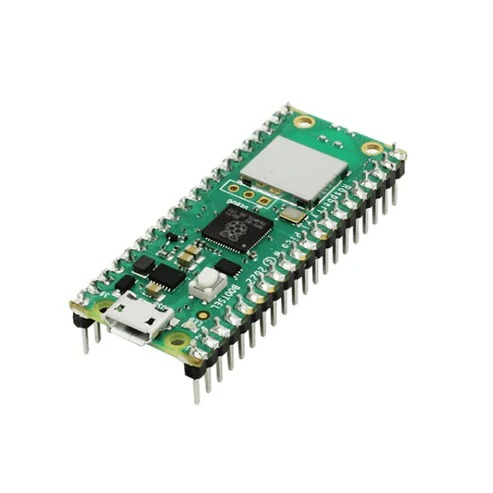
\includegraphics[width=1.16667in,height=0.95833in]{media/ras.jpeg}\\
					\caption{Raspberry Pi }
					
					\!
					\!
				\end{figure}
				\\The Pico W is based on the RP2040 microcontroller, which was designed by Raspberry Pi in-house. It combines a powerful ARM Cortex-M0+ processor with built-in Wi-Fi connectivity. The Pico W brings 802.11n wireless networking to the Pico platform, opening up a range of possibilities for IoT projects, remote monitoring, and wireless communication13. The RP2040 microcontroller features a dual-core Arm Cortex M0+ processor, flexible clock running up to 133 MHz, 264kB of SRAM, and 2MB of on-board flash memory1. The Pico W has 26 multi-function GPIO pins, 2 SPI, 2 I2C, 2 UART, 3 12-bit ADC, and 16 controllable PWM channels.
				Programmable I/O: It also features 8 Programmable I/O (PIO) state machines for custom peripheral support. The Pico W retains complete pin compatibility with its older sibling, the Raspberry Pi Pico3. Fast cores, large memory, and flexible interfacing make RP2040 a natural building block for Internet of Things (IoT) applications.
				
				
			\end{quote}
			
			\begin{quote}
				\textbf{2. Relay Module :}
				\begin{figure}[htbp]
					\centering
%					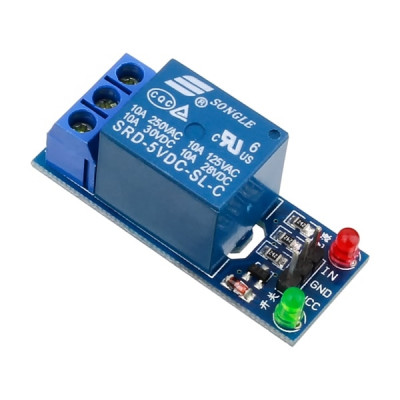
\includegraphics[width=2.16667in,height=2.95833in]{media/relay.jpeg}
					\caption{Relay Module}
				\end{figure}
				\\A relay module is an electronic device that consists of one or more relays, along with supporting components such as indicator LEDs, protection diodes, transistors, and resistors. The primary function of a relay module is to switch high voltage and current loads using low voltage signals. It serves to isolate the control circuit from the device or system being controlled. This allows the use of a microcontroller or other low-power device to control devices with much higher voltages and currents. Relay modules come in diverse shapes and sizes, with the most common configurations being rectangular boards containing 2, 4, or 8 relays. Some relay modules can house up to 16 relays. The relay module input voltage is usually DC. However, the electrical load that a relay will control can be either AC or DC, but essentially within the limit levels that the relay is designed for. A typical relay module includes pins for Normally Open (NO), Normally Closed (NC), Common Contact, and Signal Pin4. The NO and NC pins are used to connect the load, while the Signal Pin is used to control the relay. Relay modules find use in a lot of different applications, especially in systems requiring higher power than what a microcontroller can provide. They are commonly used in home automation systems, industrial machinery, and various types of electronic equipment.
			\end{quote}
			
			
			\begin{quote}
				\textbf{3. PIR Sensor :}\\
				\begin{figure}
					\centering
%					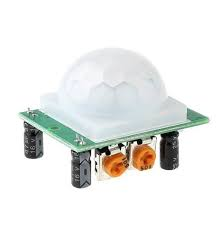
\includegraphics[width=1.16667in,height=0.95833in]{media/pir.jpeg}\\
					\caption{PIR Sensor}
				\end{figure}
				A Passive Infrared Sensor (PIR Sensor) is an electronic sensor that measures infrared (IR) light radiating from objects in its field of view. PIR sensors are most often used in PIR-based motion detectors1. They are commonly used in security alarms and automatic lighting applications. PIR sensors detect the infrared radiation generated by objects or live animals inside its range of vision, which varies in temperature from warm to cold. This change is recognized when an item travels across this field, triggering the sensor’s alert. PIR sensors are fundamentally made of a pyroelectric sensor, which can detect levels of infrared radiation. They are flat control and minimal effort, have a wide lens range, and are simple to interface with. Most PIR sensors have a 3-pin connection at the side or bottom. One pin will be ground, another will be signal and the last pin will be power. Power is usually up to 5V. PIR sensors are used in numerous essential projects or items that need to discover when an individual has left or entered the area. They are also used in all outdoor lights, lift lobbies, multi-apartment complexes, common staircases, basements or covered parking areas, shopping malls, and for garden lights.
				
			\end{quote}
			
			\begin{quote}
				\textbf{4. Jumper Wire :}\\
				\begin{figure}
					\centering
%					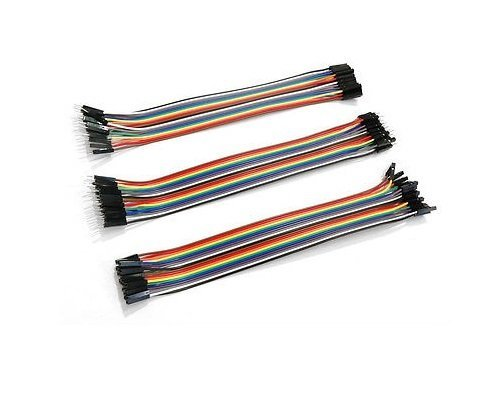
\includegraphics[width=2.16667in,height=1.95833in]{media/wire.jpg}\\
					\caption{Jumper Wire}
				\end{figure}
				A Jumper Wire, also known as a jump wire or DuPont wire, is an electrical wire with a connector or pin at each end Jumper wires are used to interconnect the components of a breadboard or other prototype or test circuit, internally or with other equipment or components, without soldering. They are typically used in DIY electrical projects. Jumper wires are simply wires that have connector pins at each end32. They come in a wide array of colors. However, the colors don’t actually mean anything and are just an aid to help you keep track of what is connected to which. Jumper wires typically come in three versions: male-to-male, male-to-female, and female-to-female. The difference between each is in the endpoint of the wire. Male ends have a pin protruding and can plug into things, while female ends do not and are used to plug things into. Jumper wires are commonly used with breadboards and other prototyping tools like Arduino. They make changing circuits as simple as possible.
				
				\begin{quote}
					\textbf{5. Breadboard :}
					\begin{figure}[htbp]
						\centering
%						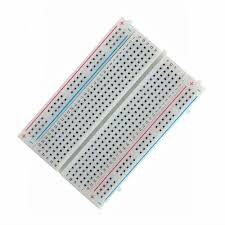
\includegraphics[width=2.16667in,height=2.95833in]{media/board.jpg}
						\caption{Breadboard}
					\end{figure}
					\\A breadboard, also known as a solderless breadboard or protoboard, is a construction base used for building semi-permanent prototypes of electronic circuits. Breadboards are typically rectangular boards containing holes into which circuit components like ICs, resistors, capacitors, and transistors can be inserted. They also have adhesive backing and many tie points (holes) into which circuit components can be inserted. The primary function of a breadboard is to construct and test circuits without soldering. The components are inserted into the breadboard’s holes and can be easily repositioned or removed, making breadboards ideal for prototyping and experimenting with circuit designs Breadboards are popular in electronics education to build and test circuits quickly. They are also used by hobbyists and professionals alike. While breadboards are convenient for prototyping, they do have limitations. They are not suitable for use with high-frequency circuits (above 10 MHz) due to the parasitic capacitance and inductance of the breadboard. Also, the connections on a breadboard are less reliable and more prone to failure compared to soldered connections. The term “breadboard” comes from the early days of electronics, when people would literally drive nails or screws into wooden boards (often used for cutting bread) on which they mounted their electronic components.
				\end{quote}
				
				\begin{quote}
					\textbf{6. Cooling Fan :}
					\begin{figure}[h]
						\centering
%						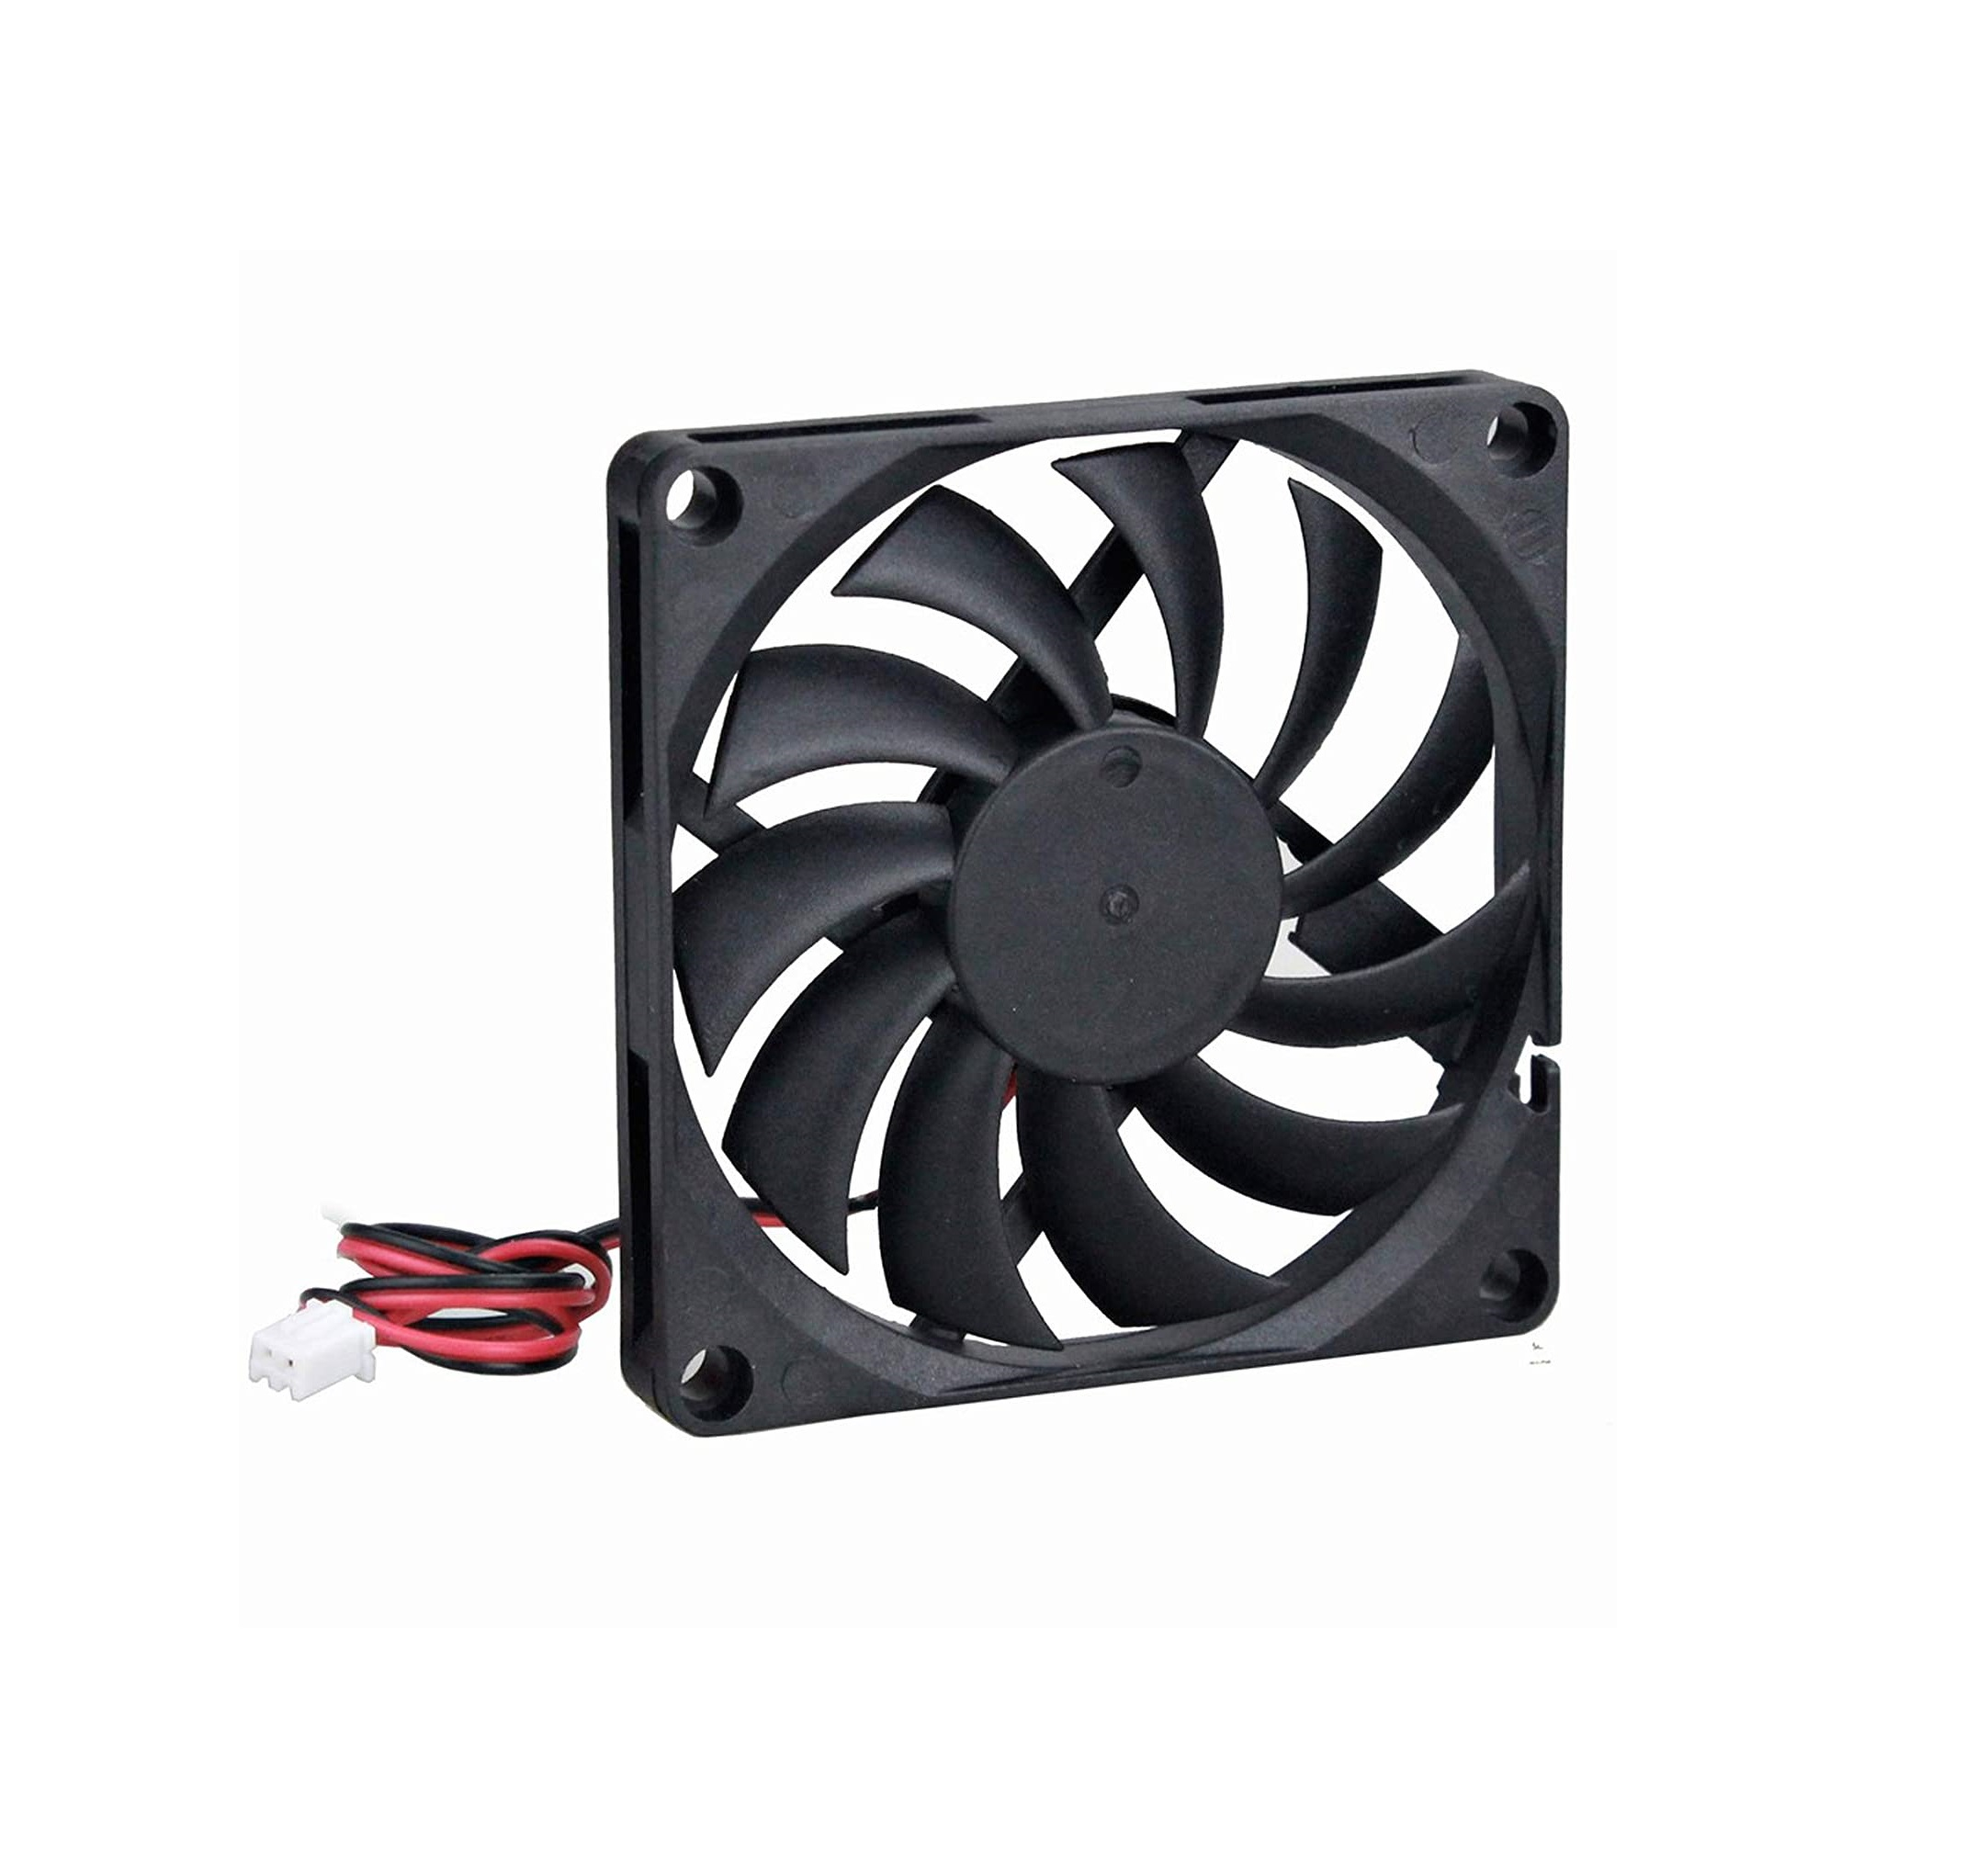
\includegraphics[width=2.16667in,height=1.95833in]{media/fan.jpg}\\
						\caption{Cooling Fan}
						
					\end{figure}
					\\A cooling fan, also known as a radiator fan, is a device designed to cool or ventilate an environment by blowing air. Typically, the fan is positioned between the radiator and the engine as it draws heat to the atmosphere. In front-wheel cars, the cooling fan used is an electrical component powered by the battery. Cooling fans are widely used in various devices such as computers, gaming consoles, and home appliances. They help to maintain an optimal temperature and prevent overheating, which could lead to performance issues or damage. There are various types of cooling fans available in the market, including tower fans, pedestal fans, floor fans, and mini portable fans. Some popular brands of cooling fans include Honeywell, Dyson, Rowenta, and Vornado.
				\end{quote}
				
			\end{quote}
			
		\end{quote}
	\end{quote}
	\clearpage
	
	
	%system diagram
	\begin{quote}
		\section{3. Design And Development}
		
		\subsection{3.1 Block Daigram}
		A block diagram is a graphical representation of a system. It provides a functional view of a system and depicts the flow of information within the system.\\
		
		\begin{quote}
			
			
			\begin{figure}
				\centering
%				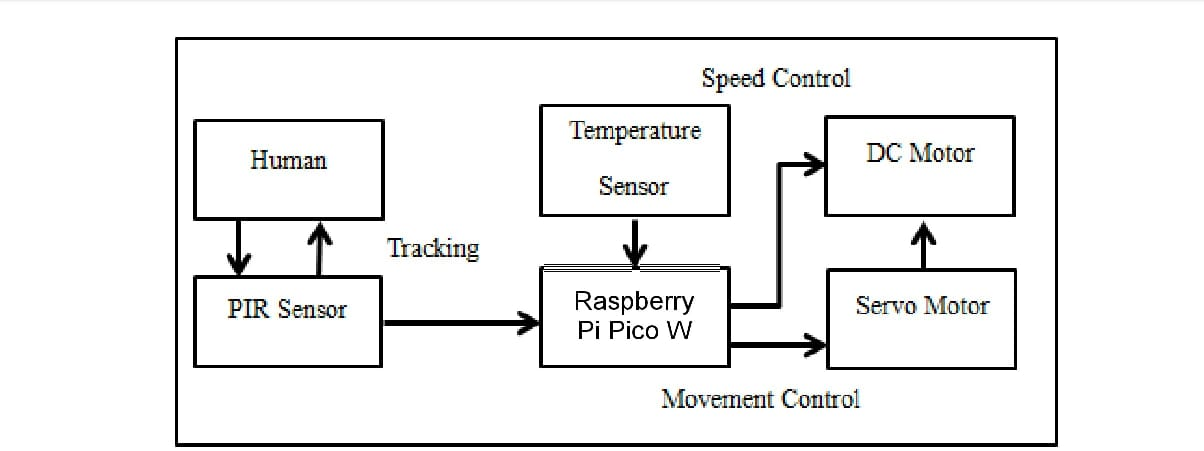
\includegraphics[width=20cm,height=15cm]{media/block.jpeg}\\
				\caption{Block Diagram}
			\end{figure}
			
		\end{quote}
		\clearpage
		\subsection{3.2 Circuit Diagram}
		Use Case Diagram focuses on the interactions between a system and external entities, known as actors. Actors can be users or external systems, while use cases represent specific functionalities or tasks the system performs. Use case diagrams are beneficial for visualizing system functionalities, identifying actors, and depicting the relationships between them.
		\begin{figure}
			\centering
%			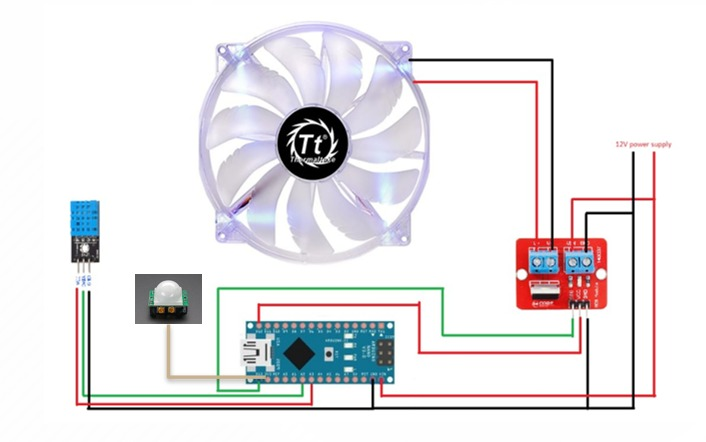
\includegraphics[width=20cm,height=10cm]{media/circuit.jpeg}\\
			\caption{Circuit Diagram}
		\end{figure}
		\clearpage
		
	\end{quote}
	\clearpage
	
	
	%specification
	\begin{quote}
		\section{4. Specification}
		\textbf{Hardware Components : }\\
		Raspeberry Pi Pico W, Relay Module, PIR Sensor, Cooling Fan, Jumper Wire, BreadBoard\\
		\vspace{0.3cm}
		\textbf{Software :  }\\
		Phonny		\\
		\vspace{0.3cm}
		\textbf{Tools Used : }\\
		\begin{quote}
			\textbf{1. Programming language :}\\Micro Python\\
			\vspace{0.2cm}
			\textbf{2. Documentation :}\\Star UML, Latex\\
		\end{quote}
	\end{quote}
	\clearpage
	
	\clearpage
	
	
	%implementation
	\begin{quote}
		\section{5. Experimentation, Result And Discussion}
%		\textbf{1. Login Page}
		\begin{figure}[h]
			\centering
%			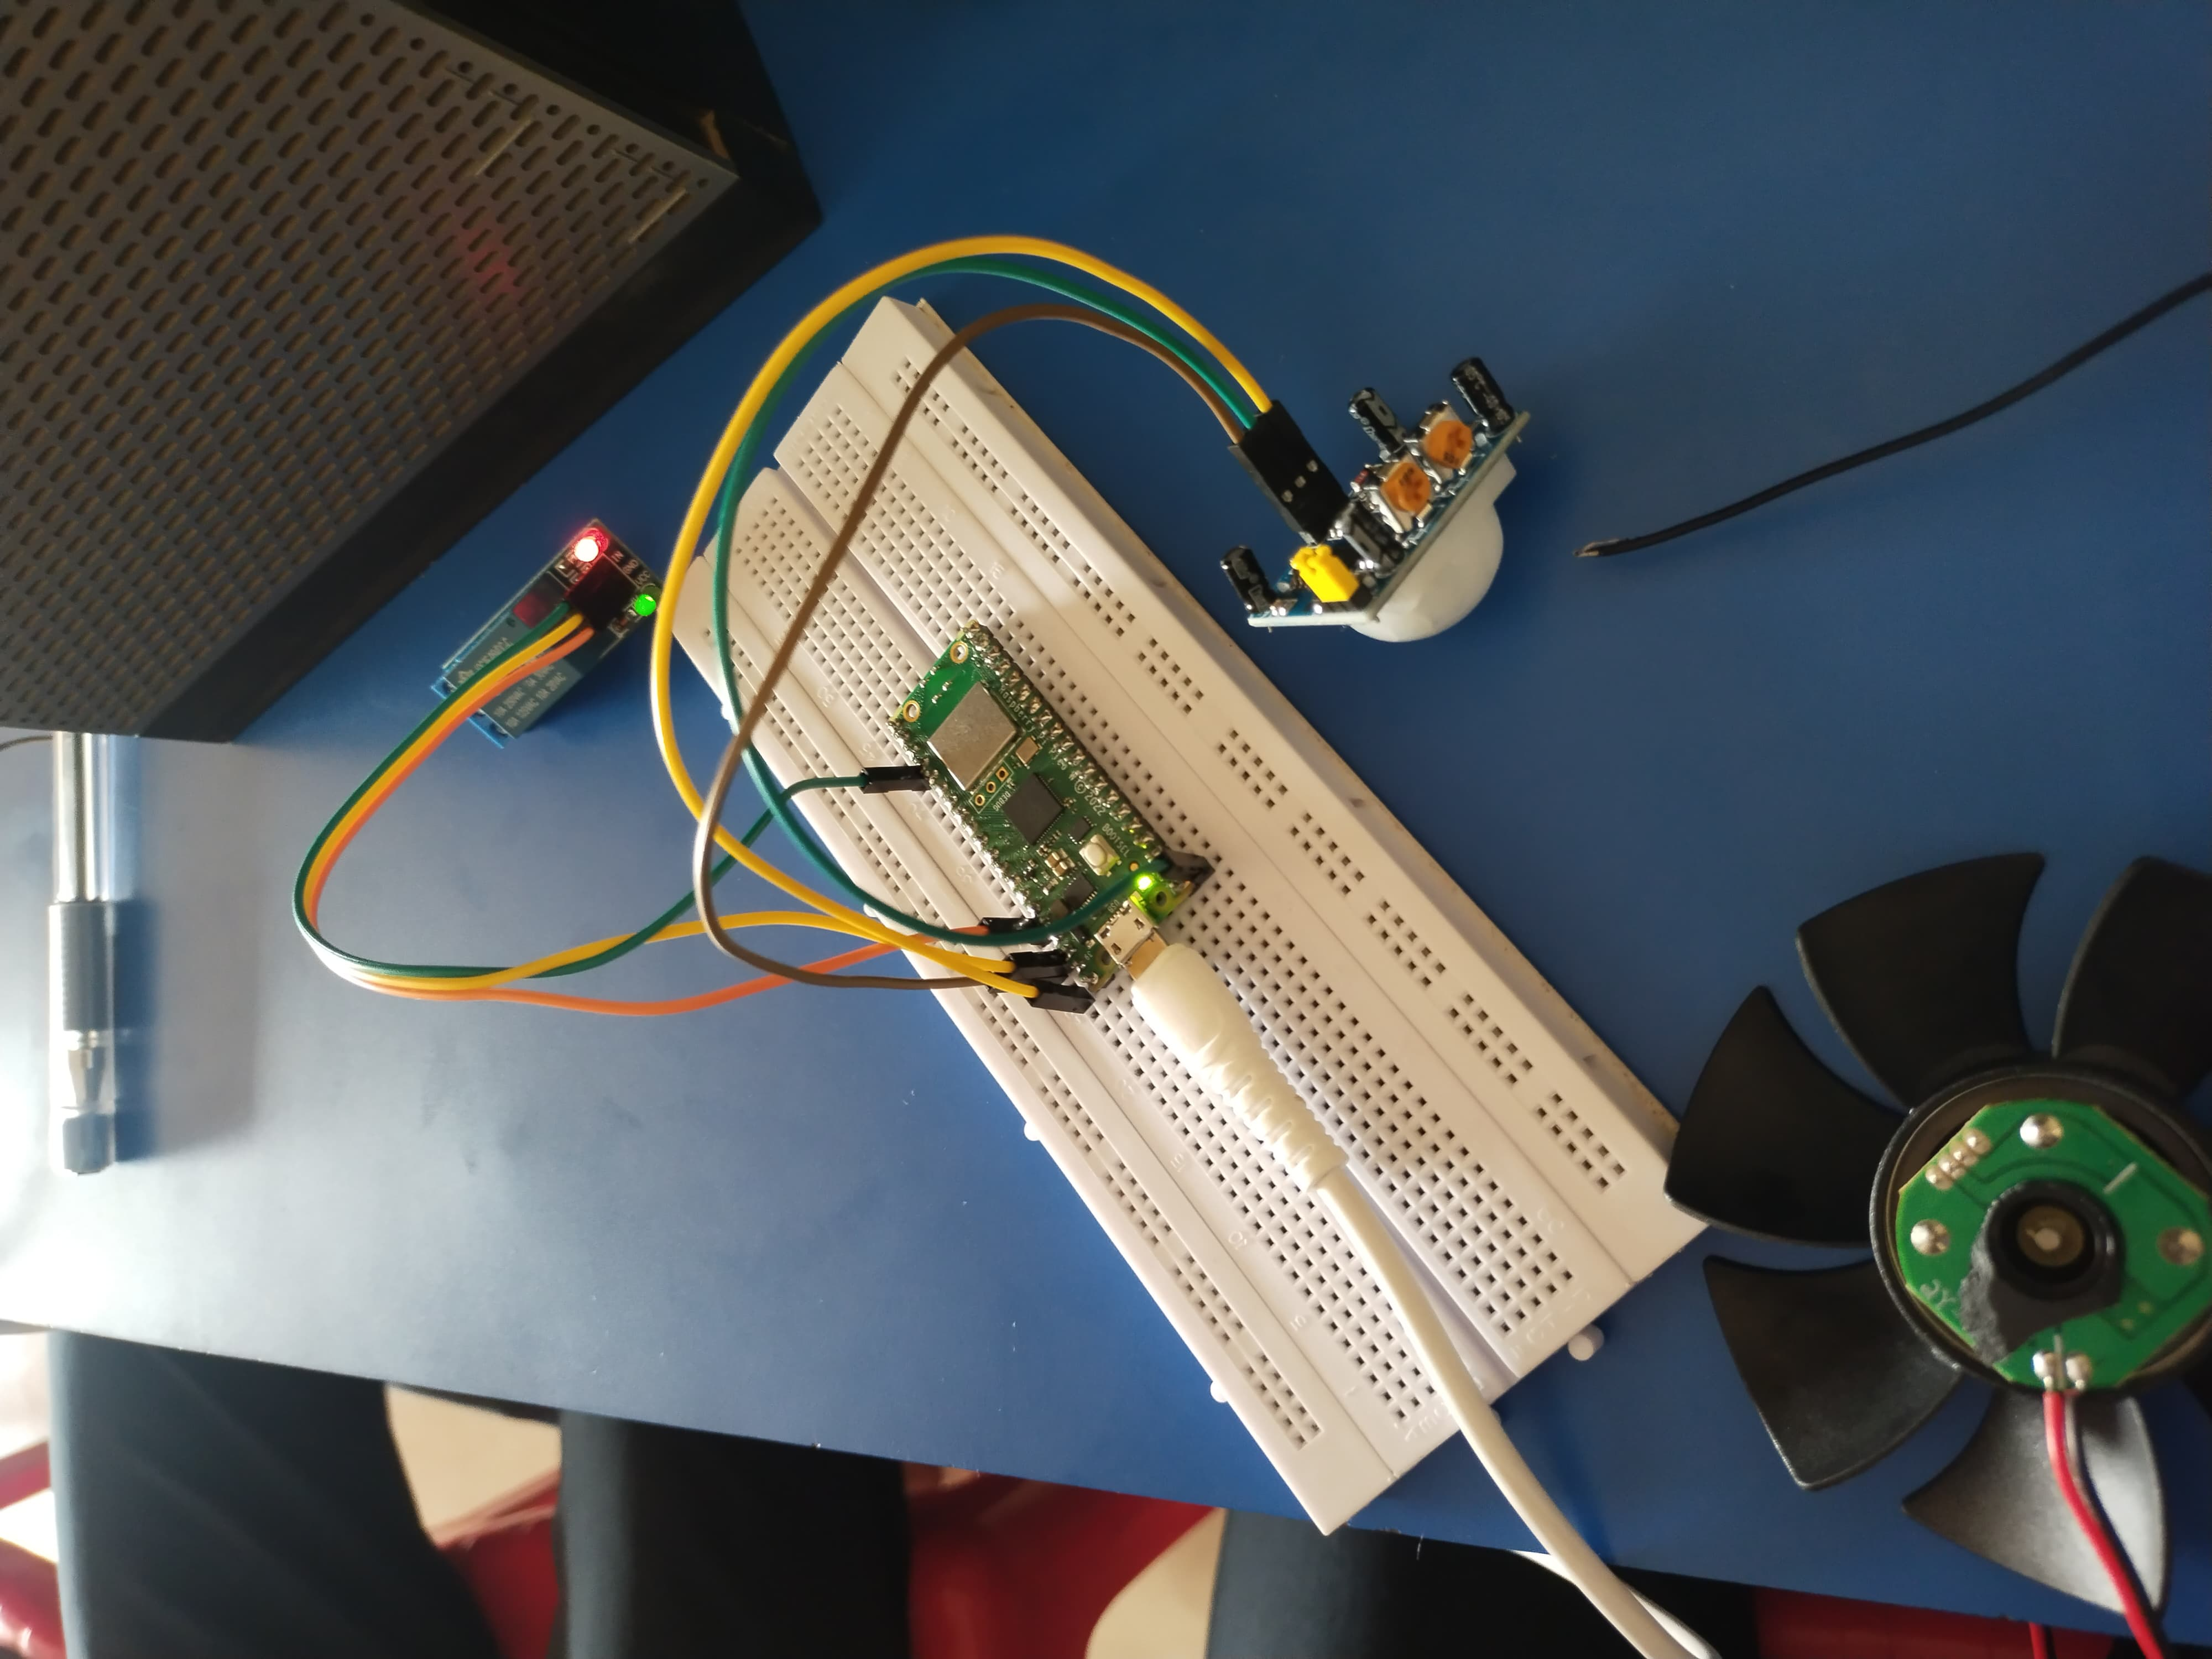
\includegraphics[width=35cm,height=10cm]{media/result.jpeg}\\
			%	\caption{}
			%	\vspace{0.5cm}	
			\paragraph{}
			\justify
			Raspberry Pi Pico W: This is the main controller of your project. 
			PIR Motion Sensor: Connect the VCC pin of the PIR sensor to the 3.3V pin on the Raspberry Pi Pico W, the GND pin to a GND pin on the Raspberry Pi Pico W, and the Data pin to a suitable GPIO pin on the Raspberry Pi Pico W. The PIR sensor will output a HIGH signal on the Data pin when it detects movement.
			Relay Module: Connect the VCC pin of the relay module to the 3.3V pin on the Raspberry Pi Pico W, the GND pin to a GND pin on the Raspberry Pi Pico W, and the Input pin to another suitable GPIO pin on the Raspberry Pi Pico W. The relay module will be used to control the power to the fan.
			Fan: Connect your fan to the Normally Open (NO) and Common (COM) terminals of the relay module. When the relay is triggered by the Raspberry Pi Pico W, it will allow power to flow to the fan.
			Battery: The battery will be used to power the Raspberry Pi Pico W. Connect the positive terminal of the battery to the VIN pin on the Raspberry Pi Pico W and the negative terminal to a GND pin.
		\end{figure}
		\clearpage
		
	\end{quote}
	\clearpage
	
	
	
	\clearpage
	
	
	\begin{quote}
		\section{6. Conclusion And Future Scope}
		\subsection{6.1 Conclusion}
		\begin{quote}
			Conclusion: The project “Automatic Fan Control Based on Motion Detection and Temperature Using Raspberry Pi Pico W” successfully integrates the concepts of Internet of Things (IoT), temperature monitoring, and motion detection to create an efficient and user-friendly system12. The system precisely measures temperature and reliably controls the fan based on the temperature and motion detected12. This not only improves user convenience and environmental comfort but also enhances energy efficiency.
		\end{quote}
		\clearpage
		\subsection{6.2 Future Scope}
		\begin{quote}
			Future Scope: The project opens up several avenues for future work. Some potential improvements and extensions could include:
			
			1. Security Enhancements: As with any IoT device, security is a crucial aspect. Future work could focus on enhancing the security of the system to protect against potential threats.
			
			2. Interaction with Other IoT Devices: The system could be designed to interact with other IoT devices in a smart home environment, providing a more integrated and seamless user experience.
			
			3. Geographical Sensing: The system could be enhanced with geographical sensing capabilities to adjust the fan speed based on the geographical location and local weather conditions.
			
			4. Adaptive Fan Speed Management: The system could incorporate machine learning algorithms to learn from the user’s preferences and adapt the fan speed accordingly.
			
			5. Reliability Improvements: Future work could also focus on improving the reliability of the system, ensuring consistent performance under various conditions.
			
			6. Integration with Renewable Energy Sources: The system could be integrated with renewable energy sources like solar power, making it more sustainable and environmentally friendly.
			
			7. These enhancements would not only improve the functionality and user experience of the system but also contribute to the broader field of IoT and home automation.
			
			
		\end{quote}
		
	\end{quote}
	\clearpage
	
	\begin{quote}
		\section{7. References}
		\justifying
		\begin{quote}
			\justifying
			1. GitHub. [https://github.com/JeremySCook/RaspberryPi-Fan-Control]
			\justifying
			
			
		\end{quote}
	\end{quote}
	
\end{document}
